\chapter{Implementacja}

W niniejszym rozdziale przedstawiono szczegóły implementacji aplikacji. Każdej ze scen poświęcono osobny podrozdział, w którym odniesiono się do wykorzystanych technologii, bibliotek oraz zrealizowanych sposobów komunikacji pomiędzy poszczególnymi elementami widoku. W projekcie zamieszczono kody funkcji realizujących najistotniejsze zadania.

\section{Struktura aplikacji}
Struktura projektu wykorzystuje domyślne ułożenie plików w systemie Unity. Jako główny folder służy folder \texttt{Assets}, zawiera on główne pliki projektowe: skrypty, tekstury, dźwięki, grafiki, prefaby(gotowe elementy często wykorzystywane w projekcie).

Pliki w folderze \texttt{Scripts} zorganizowano według ich celu. Każdy plik przypisany do danej sceny znajduje się w odpowiednim folderze (rys.~\ref{fig:strukturaKodu}). Elementy pomocnicze, jak np.\ kod pomocy kontekstowej, kod przycisku zamykania sceny, znajdują się w folderze \texttt{Utility}. 
 
\begin{figure}[htb]
     \centering
 	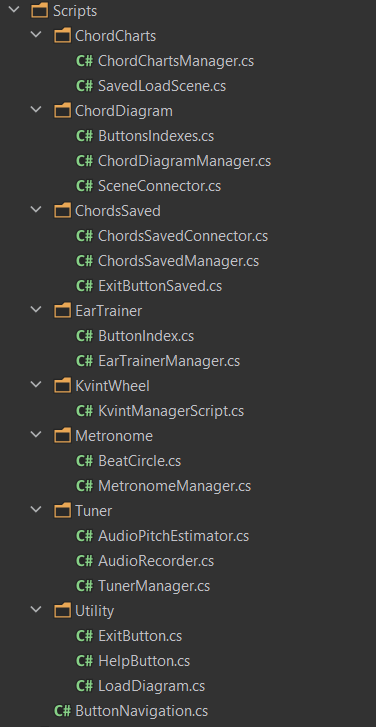
\includegraphics[scale=.8]{rys04/StrukturaPlikow}
	\caption{Struktura źródeł kodu w projekcie}
	\label{fig:strukturaKodu}
\end{figure}
% DONE: w rozdziale dobrze byłoby zamieścić opis struktury projektu. Ponieważ rozwijał Pan aplikację w środowisku UNITY, to środowisko narzuca trochę tę strukturę (parę uwag na ten temat też by się przydało). Strukturę projektu można pokazać robiąc zrzuty drzewa źródeł kodu.

% DONE: przydałoby się też opowiedzieć trochę o budowaniu aplikacji (testowe uruchomienia odbywają się w środowisku, aby można było uruchomić aplikację poza tym środowiskiem - coś trzeba przecież zrobić).
Aby na bieżąco analizować poprawność zaimplementowanych funkcji wykorzystywano wbudowaną w silnik Unity opcję \emph{play}, która umożliwia ,,odpalenie'' jednej sceny, nie wymuszając przy tym budowania całej aplikacji od nowa. Po wykryciu zmian w kodzie aplikacja się przeładowuje i jest gotowa do użycia/przetestowania przez użytkownika.

\section{Implementacja elementów aplikacji}

\subsection{Stroik}

Głównymi elementami sceny sa przyciski służące do wyboru domniemanej nuty. W skład widoku wchodzi tez jej tytuł, informator odnośnie aktualnego poziomu nastrojenia instrumentu i~przyciski odpowiedzialne za zmianę docelowego instrumentu. Do menadżera sceny przypięte zostały 3 pliki z kodem zawierające definicje klas, realizujące logikę potrzebną do nagrania, przeanalizowania i wyświetlenia wyników analizy dźwięku. Nazwy tych klas to: \texttt{AudioRecorder} - klasa odbierająca dźwięk ze sceny, \texttt{AudioPitchEstimator} - odpowiedzialna za analizę odebranego dźwięku, \texttt{TunerManager} - główna klasa realizująca logikę sceny. 

Klasa \texttt{AudioRecorder} zawiera dwa pola:
\begin{itemize}
    \item \texttt{audioSource} -- obiekt przechowujące odwołanie do wbudowanego w silnik Unity narzędzia \texttt{AudioSource}, umożliwiającego nagranie dźwięku,
    \item \texttt{duration} -- zmienna odpowiedzialna za ustalenie czasu, przez jaki mikrofon ma odbierać dźwięk z otoczenia.
\end{itemize}
Klasa ta zawiera również jedną funkcję \texttt{OnEnable}, która podczas uruchomienia zaczyna odbierać dźwięk dostarczany do mikrofonu. 

Klasa \texttt{AudioPitchEstimator}, zaczerpnięta z repozytorium \cite{AudioPitchEstimator}, % DONE: to nie jest poprawne cytowanie, proszę zrobić odpowiedni rekord w bib, a potem użyć jego klucza w \cite
służy do analizy odebranego dźwięku. Zawiera ona wymienione poniżej zmienne, na które użytkownik może wpłynąć, aby dopasować narzędzie do swoich potrzeb.
\begin{itemize}
    \item \texttt{frequencyMin} -- minimalna częstotliwość, jaka ma być analizowana,
    \item \texttt{frequencyMax} -- maksymalna częstotliwość poddawana analizie,
    \item \texttt{harmonicsToUse} -- ilość harmonicznych jakie mają być brane pod uwagę, podczas ustalania końcowej częstotliwości odebranego dźwięku,
    \item \texttt{smoothingWidth} -- pasmo częstotliwości filtra wygładzającego widmo,
    \item \texttt{thresholdSRH} -- wartość graniczna decybeli, od której dźwięk ma być wzięty pod analizę.
\end{itemize}

Funkcją uruchamiającą szybką transformatę Fouriera na odebranym dźwięku jest \texttt{Estimate} (listing~\ref{lst:1}) z tej klasy. Zwraca one zmienną float \texttt{bestFreq}, będąca najlepszym możliwym według programu ,,trafieniem'', jeżeli chodzi o odebraną częstotliwość. Klasa \texttt{TunerManager} odpowiedzialna za realizowanie logiki sceny, przechowuje odwołania do komponentów sceny: przyciski, pola tekstowe, obiekt \texttt{AudioSource}. W jej skład wchodzi 6 funkcji o nazwie \texttt{SetDesiredFrequency*}, przy czym każdemu z przycisków przypisany jest jeden jej odpowiednik, ustawiający parametry skryptu \texttt{AudioPitchEstimator}. Funkcją odpowiedzialną za logikę analizy dźwięku jest \texttt{EstimatePitch}, która korzysta z klasy \texttt{AudioPitchEstimator}, na tej podstawia ustawia wartości elementów tekstowych informujących użytkownika o poziomie nastrojenia instrumentu. 
% TO DO:zamienione linie kodu
% var nyquistFreq = AudioSettings.outputSampleRate / 2.0f;
% if (!audioSource.isPlaying) return float.NaN;

\begin{lstlisting}[style=sharpcstyle,caption=Funkcja \texttt{Estimate}, label=lst:1]
public float Estimate(AudioSource audioSource)
{
    if (!audioSource.isPlaying) return float.NaN;
		var nyquistFreq = AudioSettings.outputSampleRate / 2.0f;
    audioSource.GetSpectrumData(spectrum, 0, FFTWindow.Hanning);

    for (int i = 0; i < spectrumSize; i++)
    {       
        specRaw[i] = Mathf.Log(spectrum[i] + 1e-9f);
    }

    specCum[0] = 0;
    for (int i = 1; i < spectrumSize; i++)
    {
        specCum[i] = specCum[i - 1] + specRaw[i];
    }

    var halfRange = Mathf.RoundToInt((smoothingWidth / 2) / nyquistFreq * spectrumSize);
    for (int i = 0; i < spectrumSize; i++)
    {    
        var indexUpper = Mathf.Min(i + halfRange, spectrumSize - 1);
        var indexLower = Mathf.Max(i - halfRange + 1, 0);
        var upper = specCum[indexUpper];
        var lower = specCum[indexLower];
        var smoothed = (upper - lower) / (indexUpper - indexLower);        
        specRes[i] = specRaw[i] - smoothed;
    }

    float bestFreq = 0, bestSRH = 0;
    for (int i = 0; i < outputResolution; i++)
    {
        var currentFreq = (float)i / (outputResolution - 1) * (frequencyMax - frequencyMin) + frequencyMin;       
        var currentSRH = GetSpectrumAmplitude(specRes, currentFreq, nyquistFreq);
        for (int h = 2; h <= harmonicsToUse; h++)
        {
           currentSRH += GetSpectrumAmplitude(specRes, currentFreq * h, nyquistFreq);
           currentSRH -= GetSpectrumAmplitude(specRes, currentFreq * (h - 0.5f), nyquistFreq);
        }
        srh[i] = currentSRH;
       
        if (currentSRH > bestSRH)
        {
            bestFreq = currentFreq;
            bestSRH = currentSRH;
        }
    }
    
    if (bestSRH < thresholdSRH) return float.NaN;

    return bestFreq;
}
\end{lstlisting}

\begin{itemize}
    \item \texttt{Start} -- funkcja przypisująca przyciskom im działania w wypadku naciśnięcia.
    \item \texttt{ClearColor} -- funkcja pomocnicza, odpowiedzialna za ,,czyszczenie'' elementów graficznych sceny.
\end{itemize}

\subsection{Metronom}

Scena metronomu zawiera 4 przyciski służące do parametryzacji działania metronomu, umożliwiając zwiększenie tempa, zwiększanie lub zmniejszanie liczby taktów. Za logikę odpowiada menadżer sceny z przypiętą klasą \texttt{MetronomeManager}, zawierająca 5 pól obiektów przycisków, pole obiektu tekstowego i kilka zmiennych pomocniczych. Metronom realizowany jest za pomocą wizualizacji poszczególnych taktów za pomocą graficznych elementów w postaci "kółek", które dodawane są do widoku dynamicznie w zależności od ustalonych przez użytkownika wartości. Funkcje jakie implementuje dana klasa to:

\begin{itemize}
    \item \texttt{Start} -- funkcja odpowiadająca za ustawienie zmiennych, obiektów widoku. 
    \item \texttt{AddCircle} -- funkcja wykorzystywana do zwiększenia tempa.
    \item \texttt{DeleteCircle} -- funkcja wykorzystywana do zmniejszenia tempa.
    \item \texttt{RearrangeElements} -- funkcja stworzona do rozmieszczania ,,kółek'' taktów na ekranie.
    \item \texttt{StartMetronome} -- funkcja uaktywniająca metronom.
    \item \texttt{RecolorAll} -- funkcja uruchamiana podczas resetu metronomu, czyszcząca grafiki wizualizacji metronomu.
    \item \texttt{MetronomeCoroutine} -- osobny wątek odpowiedzialny za działanie metronomu, w czasie działania tej funkcji wybijane jest na ekranie tempo.
    \item \texttt{AddBpm} -- funkcja odpowiedzialna za zwiększenie tempa.
    \item \texttt{SubtractBpm} -- funkcja odpowiedzialna za zmniejszenie tempa.
\end{itemize}

Za główną logikę sceny odpowiada funkcja \texttt{MetronomeCoroutine} (listing~\ref{lst:2}). Odgrywa ona dźwięk oznaczający kolejny takt metronomu i zmienia kolory odpowiednich przycisków.

\begin{lstlisting}[style=sharpcstyle,caption=Wątek \texttt{MetronomeCoroutine}, label=lst:2]
IEnumerator MetronomeCoroutine()
{
    float beatDuration = 60f / bpm;
    float noteDuration;
    noteDuration = beatDuration;
    int currentIndex = 0;
    int previousIndex = -1;

    while (true)
    {
        if (circles.Count > 0)
        {
            audioSource.Play();
            
            if (previousIndex != -1 && previousIndex < circles.Count)
            {
                circles[previousIndex].GetComponent<BeatCircle>().changeColorWhite();
            }
            
            var currentCircle = circles[currentIndex].GetComponent<BeatCircle>();
            if (currentCircle.imgComponent.color == Color.black)
            {
                currentCircle.changeColorWhite();
            }
            else
            {
                currentCircle.changeColorBlack();
            }

            previousIndex = currentIndex;
            currentIndex = (currentIndex + 1) % circles.Count;
        }
        
        yield return new WaitForSeconds(noteDuration);
    }
}
\end{lstlisting}

\subsection{Księga akordów}
%DONE : zrobić odwołania poprawne do listingów takie jak w zaleceniach
Scena księgi akordów zawiera element graficzny reprezentujący aktualnie wybrany akord gitarowy, przyciski umożliwiające wybór docelowego akordu, elementy graficzne ułatwiające nawigację po widoku sceny. Funkcje wchodzące w~skład klasy menadżera sceny nazwanego \texttt{ChordChartsManager} to:

\begin{itemize}
    \item \texttt{Start} -- funkcja odpowiedzialna za przygotowanie potrzebnych elementów sceny. Przypisuje grafiki akordów z pomocniczej listy \texttt{Chords} do listy głównej \texttt{ch}. Ustawia wartości zmiennych n\texttt{oteIterator},\texttt{ variantIterator} z wartości przechowywanych w skrypcie \texttt{SceneConnector}, łączącej scenę księgi akordów z widokiem wszystkich akordów w postaci diagramu. Przypisuje ona funkcje do odpowiednich przycisków i resetuje wartości obiektów tekstowych.
    \item \texttt{noteIncrement} -- funkcja przypisana do przycisku, odpowiedzialna za zmianę nuty akordu.
    \item \texttt{noteDecrement} -- funkcja przypisana do przycisku, odpowiedzialna za zmianę nuty akordu.
    \item \texttt{variantIncrement} -- funkcja przypisana do przycisku, odpowiedzialna za zmianę wariacji akordu.
    \item \texttt{variantDecrement} -- funkcja przypisana do przycisku, odpowiedzialna za zmianę wariacji akordu.
    \item \texttt{ChangeVariantText} -- funkcja odpowiedzialna za zmianę przypisanej wartości obiektu tekstowego sceny, wykorzystywana w momencie zmiany wariacji akordu.
    \item \texttt{ChangeNoteText} -- funkcja odpowiedzialna za zmianę przypisanej wartości obiektu tekstowego sceny, wykorzystywana w momencie zmiany nuty akordu.
    \item \texttt{ChangeChord} -- funkcja odpowiedzialna za zmianę aktualnie wyświetlanego akordu, zmienia przypisaną grafikę obiektu \texttt{Image} sceny.
\end{itemize}

Istotną funkcją jest \texttt{ChangeChord} (\ref{lst:3}), która odpowiada za zmianę wyświetlanej grafiki. Wewnątrz funkcji z racji sposobu zapisu grafik jako pliki .png, nie obsługiwanych domyślnie przez silnik Unity, tworzone są wpierw tekstury, na podstawie których tworzone są \emph{sprity}. Te przypisywane są do elementu graficznego znajdującego się na scenie.

\begin{lstlisting}[style=sharpcstyle,caption=Funkcja \texttt{ChangeChord}, label=lst:3]
private void ChangeChord()
{
    Texture2D selectedTexture = ch[noteIterator][variantIterator];
    Sprite newSprite = Sprite.Create(selectedTexture, new Rect(0, 0, selectedTexture.width, selectedTexture.height), new Vector2(0.5f, 0.5f));        
    chordImage.sprite = newSprite;        
    image.sprite = newSprite;
}
\end{lstlisting}

\subsection{Trening słuchu}

Scena treningu słuchu zawiera przycisk odpowiedzialny za wybór skali. W skład sceny wchodzą dwie klasy: \texttt{EarTrainerManager} -- przypisany do menadżera sceny realizujący główną logikę sceny oraz \texttt{ButtonIndex} -- klasa pomocnicza przypisana do każdego z przycisków odpowiedzialnych za udzielenie odpowiedzi. Funkcje wchodzące w~skład głównej klasy to:
\begin{itemize}
    \item \texttt{Start} -- funkcja przypisująca obiekt \texttt{audioSource}, odpowiedzialny za odgrywanie dźwięków. Ustawia ona również funkcję \texttt{PlayRandomNote} do przycisku \texttt{playNoteButton}. Dodatkowo przypisuje ona funkcję \texttt{NoteGuessed} do każdego z przycisków odpowiedzialnych za odpowiedź.
    \item \texttt{PlayRandomNote} -- funkcja odpowiedzialna za odegranie losowego dźwięku po naciśnięciu przycisku \texttt{playNoteButton}. Ustawia ona odpowiedni index dla odegranej nuty, wykorzystywany następnie podczas zweryfikowania odpowiedzi podanej przez użytkownika.
    \item \texttt{NoteGuessed} -- funkcja weryfikująca odpowiedź użytkownika. Ustawia ona obiekty tekstowe sceny, w zależności od tego czy odpowiedź była poprawna, czy też nie. 
    \item \texttt{DeactivateObjects} -- funkcja odpowiedzialna za wyłączenie obiektów graficznych sceny.
    \item \texttt{ResetTraining} -- funkcja dezaktywująca aktualny trening, przenosząc użytkownika do widoku początkowego.
    \item \texttt{SelectedScaleTreining*} -- funkcje odpowiadające za ustawienie parametrów sceny w zależności od wybranej skali treningu.
\end{itemize}

Za odegranie nuty, a następnie sprawdzenia poprawności odpowiedzi odpowiedzialny jest główna klasa (listing~\ref{lst:4}).

\begin{lstlisting}[style=sharpcstyle,caption=Funkcje \texttt{PlayRandomNote} i \texttt{NoteGuessed}, label=lst:4]
void PlayRandomNote()
{
    feedbackText.text = "Odgadnij"; 
    correctNoteIndex = Random.Range(0, noteClips.Count);
    
    audioSource.clip = noteClips[correctNoteIndex];
    audioSource.Play();
}

void NoteGuessed(Button button)
{
   if (button.GetComponent<ButtonIndex>().buttonNumber == correctNoteIndex)
   {
       feedbackText.text = "poprawnie";
   }
   else
   {
       feedbackText.text = "niepoprawna odpowiedź";
   }
}
\end{lstlisting}

Klasa pomocnicza przechowuje jedynie jedną zmienną, wykorzystywaną w momencie weryfikacji odpowiedzi udzielonej przez użytkownika, jest nią: \texttt{buttonNumber}.

\subsection{Koło kwintowe}

Scena koła kwintowego zawiera 24 przyciski, każdemu z nich przypisana została odpowiednia nuta. W kodzie menadżera sceny utworzone zostały dwie listy, przechowujące przyciski koła zewnętrznego oraz koła wewnętrznego. Kod zawiera w sobie 6 funkcji:

\begin{itemize}
\item \texttt{Start} -- funkcja używana podczas tworzenia obiektu, służy ona przygotowaniu wszystkich przycisków oraz przypisania im działania przy ich naciśnięciu, w tym przypadku przypisuje ich działanie do funkcji \texttt{DisplayScale}
\item \texttt{DisplayScale} -- funkcja odpowiedzialna jest za wyświetlenie skali majorowej, oraz 3 akordów minorowych pasujących do wybranej przez użytkownika nuty. 
\item \texttt{GetColorTint} -- funkcja pomocnicza generująca kolejne odcienie kolorów, dla funkcji \texttt{DisplayScale}.
\item \texttt{GetMajorScaleIndices} -- funkcja pomocnicza generująca interwały kolejnych nut w skali majorowej.
\item \texttt{ChangeButtonColor} -- funkcja pomocnicza odpowiedzialna za zmianę koloru odpowiedniego przycisku.
\item \texttt{ClearColors} -- funkcja pomocnicza czyszcząca kolory wszystkich przycisków.
\end{itemize}

Najistotniejsza funkcja, czyli \texttt{DisplayScale} zademonstrowano poniżej (\ref{lst:5}), pominięta część funkcji to fragment kodu odpowiedzialny jedynie za zmianę koloru odpowiednich elementów.

\begin{lstlisting}[style=sharpcstyle,caption=Funkcja \texttt{DisplayScale}, label=lst:5]
public void DisplayScale(int noteIndex)
{
    ClearColors();

    List<int> scaleIndices = GetMajorScaleIndices(noteIndex);

    for (int i = 0; i < scaleIndices.Count; i++)
    {
        int index = scaleIndices[i];
        if (index < outerButtons.Count)
        {
            Color tint = GetColorTint(i);
            ChangeButtonColor(outerButtons[index], tint);
        }
    }
    ...         
}
\end{lstlisting}

\section{Diagram akordów}

Diagram akordów jest widokiem, do którego można dostać się jedynie ze sceny księgi akordów. Przedstawia on wszystkie akordy zawarte w księdze akordów, aczkolwiek w widoku ogólnym. Funkcje jakie zawiera klasa głównego menadżera sceny odpowiedzialne są za uaktywnianie i dezaktywowanie poszczególnych widoków akordów.

\begin{itemize}
    \item \texttt{DiagramNextPage} -- funkcja służąca do przewijania aktualnie wyświetlanych akordów
    \item \texttt{DiagramPreviousPage} -- funkcja służąca do przewijania aktualnie wyświetlanych akordów
    \item \texttt{UpdateDiagramDisplay} -- funkcja służąca do aktualizacji aktualnie wyświetlanych akordów
    \item \texttt{DiagramSelected} -- Funkcja odpowiedzialna za zapis wybranego akordu i przekazanie informacji do księgi akordów.
\end{itemize}